% !TEX root = ../memoire.tex
\chapter{Schémas Numériques pour la Modélisation du Trafic}
\label{chap:schemas_numeriques}

\section{Introduction aux Méthodes Numériques pour les Lois de Conservation Hyperboliques}
\label{sec:intro_methodes_numeriques}

Dans ce chapitre, nous présentons les méthodes numériques développées pour résoudre efficacement les systèmes d'équations aux dérivées partielles hyperboliques issus de notre modélisation du trafic routier au Bénin. La résolution numérique de ces équations pose plusieurs défis spécifiques, notamment:
\begin{itemize}
    \item La présence de discontinuités (ondes de choc) nécessitant des méthodes adaptées
    \item Le couplage entre classes de véhicules dans notre modèle multiclasse
    \item Les variations spatiales du coefficient de ralentissement $\lambda_i(x)$
    \item Les termes sources aux intersections et autres singularités du réseau routier
\end{itemize}

Après avoir rappelé les fondements théoriques essentiels, nous présenterons une extension du schéma de Godunov spécifiquement adaptée à notre modèle multiclasse. Nous analyserons ensuite rigoureusement la stabilité et la convergence de notre méthode, ainsi que son traitement des discontinuités spatiales.

\section{Fondements Théoriques des Schémas Numériques pour le Modèle LWR}
\label{sec:fondements_schemas}

\subsection{Problématique de la Discrétisation des Lois de Conservation}
\label{subsec:problematique_discretisation}

Rappelons que notre modèle multiclasse est décrit par le système d'équations:
\begin{equation}
\frac{\partial $\rho$_i}{\partial t} + \frac{\partial ($\rho$_i v_i)}{\partial x} = S_i(x,t), \quad i \in \{1,...,N\}
\end{equation}

Il s'agit d'un système de lois de conservation hyperboliques avec termes sources. Sa résolution numérique doit respecter plusieurs propriétés fondamentales:

\begin{itemize}
    \item \textbf{Conservation}: La masse (nombre de véhicules) doit être exactement conservée
    \item \textbf{Cohérence}: La solution numérique doit converger vers une solution faible de l'équation continue lorsque les pas de discrétisation tendent vers zéro
    \item \textbf{Stabilité}: Le schéma ne doit pas amplifier les erreurs d'arrondi ou créer d'oscillations non physiques
    \item \textbf{Sélection de la solution entropique}: En présence de discontinuités, le schéma doit sélectionner la solution physiquement correcte
\end{itemize}

\subsection{Schémas Conservatifs et Théorème de Lax-Wendroff}
\label{subsec:schemas_conservatifs}

\begin{definition}[Schéma conservatif]
Un schéma numérique pour une loi de conservation est dit conservatif s'il peut s'écrire sous la forme:
\begin{equation}
$\rho$_i^{n+1} = $\rho$_i^n - \frac{$\Delta$ t}{$\Delta$ x}\left(F_{i+\frac{1}{2}} - F_{i-\frac{1}{2}}\right)
\end{equation}
où $F_{i+\frac{1}{2}}$ est un flux numérique à l'interface entre les cellules $i$ et $i+1$.
\end{definition}

\begin{theorem}[Lax-Wendroff]
Si un schéma conservatif converge, alors il converge vers une solution faible de l'équation aux dérivées partielles.
\end{theorem}

Ce théorème justifie l'utilisation de schémas conservatifs pour les problèmes de trafic, où la conservation du nombre de véhicules est une propriété physique fondamentale.

\subsection{Condition d'Entropie et Capture des Ondes de Choc}
\label{subsec:condition_entropie}

En présence de discontinuités, les solutions faibles ne sont pas uniques. Une condition supplémentaire, la condition d'entropie, est nécessaire pour sélectionner la solution physiquement pertinente.

\begin{definition}[Paire d'entropie]
Une paire $(U, F)$ est une paire d'entropie pour la loi de conservation $\partial_t $\rho$ + \partial_x f($\rho$) = 0$ si:
\begin{itemize}
    \item $U($\rho$)$ est convexe (entropie mathématique)
    \item $U'($\rho$) \cdot f'($\rho$) = F'($\rho$)$ (relation de compatibilité)
\end{itemize}
\end{definition}

\begin{theorem}[Condition d'entropie de Kruzhkov]
La solution entropique d'une loi de conservation scalaire satisfait, pour toute paire d'entropie $(U,F)$:
\begin{equation}
\partial_t U($\rho$) + \partial_x F($\rho$) \leq 0
\end{equation}
au sens des distributions.
\end{theorem}

Les schémas numériques doivent être conçus pour respecter cette condition d'entropie discrète, garantissant ainsi la sélection de la solution physique correcte.

\section{Le Schéma de Godunov et son Extension Multiclasse}
\label{sec:schema_godunov}

\subsection{Le Schéma de Godunov Standard}
\label{subsec:godunov_standard}

Le schéma de Godunov \cite{godunov1959finite} est particulièrement adapté à la résolution des lois de conservation hyperboliques. Sa philosophie est de considérer les valeurs numériques comme des moyennes sur des cellules et de résoudre exactement des problèmes de Riemann aux interfaces entre ces cellules.

Pour une équation de conservation scalaire $\partial_t $\rho$ + \partial_x f($\rho$) = 0$, le schéma s'écrit:

\begin{equation}
$\rho$_i^{n+1} = $\rho$_i^n - \frac{$\Delta$ t}{$\Delta$ x} \left( F_{i+\frac{1}{2}}^n - F_{i-\frac{1}{2}}^n \right)
\end{equation}

où le flux numérique $F_{i+\frac{1}{2}}^n$ est obtenu en résolvant exactement le problème de Riemann à l'interface:

\begin{equation}
F_{i+\frac{1}{2}}^n = f\left($\rho$^*\left($\rho$_i^n, $\rho$_{i+1}^n\right)\right)
\end{equation}

avec $\rho^*$ la valeur de $\rho$ à l'interface au temps $t^n$, obtenue par la résolution exacte du problème de Riemann.

Pour un diagramme fondamental strictement concave (comme celui de Greenshields), ce flux s'exprime:

\begin{equation}
F_{i+\frac{1}{2}}^n = 
\begin{cases} 
\min_{$\rho$ \in [$\rho$_i^n, $\rho$_{i+1}^n]} f($\rho$) & \text{si } $\rho$_i^n \leq $\rho$_{i+1}^n \\
\max_{$\rho$ \in [$\rho$_{i+1}^n, $\rho$_i^n]} f($\rho$) & \text{si } $\rho$_i^n > $\rho$_{i+1}^n
\end{cases}
\end{equation}

\begin{theorem}[Propriétés du schéma de Godunov]
Le schéma de Godunov possède les propriétés suivantes:
\begin{itemize}
    \item Il est conservatif
    \item Il est d'ordre 1 en espace et en temps
    \item Il satisfait une inégalité d'entropie discrète
    \item Il converge vers la solution entropique si la condition CFL est satisfaite
\end{itemize}
\end{theorem}

\subsection{Extension au Système Multiclasse}
\label{subsec:extension_multiclasse}

Pour notre système multiclasse couplé, l'extension directe du schéma de Godunov n'est pas triviale en raison du couplage entre les classes via la vitesse $v_i(\boldsymbol{$\rho$}, x)$. Nous avons développé une extension qui préserve les propriétés essentielles du schéma original.

Pour chaque classe $i \in \{1,\ldots,N\}$, nous appliquons le schéma:

\begin{empheq}[box=\colorbox{lightblue!15}]{align}
$\rho$_{i,j}^{n+1} = $\rho$_{i,j}^{n} - \frac{$\Delta$ t}{$\Delta$ x} \left(F_{i,j+\frac{1}{2}}^n - F_{i,j-\frac{1}{2}}^n\right) + $\Delta$ t \cdot S_i(x_j, t^n)
\label{eq:schema_godunov_multiclasse}
\end{empheq}

La difficulté réside dans le calcul du flux numérique $F_{i,j+\frac{1}{2}}^n$. Nous proposons un solveur de Riemann approché qui prend en compte le couplage entre classes:

\begin{align}
F_{i,j+\frac{1}{2}}^n = \mathcal{F}_i\left(\boldsymbol{$\rho$}^n_j, \boldsymbol{$\rho$}^n_{j+1}, x_{j+\frac{1}{2}}\right)
\end{align}

Ce flux est calculé en plusieurs étapes:

\begin{enumerate}
    \item Calcul des densités totales: $\rho_j^n = \sum_{k=1}^N $\rho$_{k,j}^n$ et $\rho_{j+1}^n = \sum_{k=1}^N $\rho$_{k,j+1}^n$
    \item Calcul des vitesses: $v_{i,j}^n = v_i(\boldsymbol{$\rho$}_j^n, x_j)$ et $v_{i,j+1}^n = v_i(\boldsymbol{$\rho$}_{j+1}^n, x_{j+1})$
    \item Application du solveur HLL (Harten-Lax-van Leer) adapté au système:
    \begin{equation}
    \mathcal{F}_i = 
    \begin{cases}
    $\rho$_{i,j}^n v_{i,j}^n & \text{si } 0 \leq S_L \\
    \frac{S_R $\rho$_{i,j}^n v_{i,j}^n - S_L $\rho$_{i,j+1}^n v_{i,j+1}^n + S_L S_R ($\rho$_{i,j+1}^n - $\rho$_{i,j}^n)}{S_R - S_L} & \text{si } S_L < 0 < S_R \\
    $\rho$_{i,j+1}^n v_{i,j+1}^n & \text{si } S_R \leq 0
    \end{cases}
    \end{equation}
\end{enumerate}

où $S_L$ et $S_R$ sont des approximations des vitesses d'onde les plus rapides à gauche et à droite, définies par:

\begin{align}
S_L &= \min(v_{i,j}^n - \sqrt{\beta_i $\rho$_{i,j}^n \left|\frac{\partial v_i}{\partial $\rho$_i}(\boldsymbol{$\rho$}_j^n, x_j)\right|}, v_{i,j+1}^n - \sqrt{\beta_i $\rho$_{i,j+1}^n \left|\frac{\partial v_i}{\partial $\rho$_i}(\boldsymbol{$\rho$}_{j+1}^n, x_{j+1})\right|}) \\
S_R &= \max(v_{i,j}^n + \sqrt{\beta_i $\rho$_{i,j}^n \left|\frac{\partial v_i}{\partial $\rho$_i}(\boldsymbol{$\rho$}_j^n, x_j)\right|}, v_{i,j+1}^n + \sqrt{\beta_i $\rho$_{i,j+1}^n \left|\frac{\partial v_i}{\partial $\rho$_i}(\boldsymbol{$\rho$}_{j+1}^n, x_{j+1})\right|})
\end{align}

avec $\beta_i$ un paramètre de classe qui contrôle la diffusion numérique.

\begin{theorem}[Propriétés du schéma multiclasse]
Le schéma étendu préserve les propriétés fondamentales suivantes:
\begin{itemize}
    \item Conservation de la masse pour chaque classe
    \item Positivité de la solution (les densités restent non négatives)
    \item Satisfaction d'une inégalité d'entropie appropriée pour le système
\end{itemize}
\end{theorem}

\begin{proof}
La conservation de la masse découle directement de la forme conservative du schéma. La positivité peut être démontrée sous une condition CFL appropriée. L'inégalité d'entropie est satisfaite par construction du solveur HLL. Les détails complets sont fournis dans l'Annexe \ref{annexe:demonstrations}.
\end{proof}

\section{Analyse de Stabilité et Condition CFL}
\label{sec:stabilite_cfl}

\subsection{Analyse de Von Neumann pour le Système Linéarisé}
\label{subsec:analyse_von_neumann}

Une analyse classique de la stabilité du schéma numérique consiste à étudier la propagation des erreurs par l'analyse de Von Neumann. En linéarisant le système autour d'un état homogène $\boldsymbol{$\rho$}_0$, on obtient:

\begin{equation}
\frac{\partial \delta\boldsymbol{$\rho$}}{\partial t} + \mathbf{A}(\boldsymbol{$\rho$}_0, x) \frac{\partial \delta\boldsymbol{$\rho$}}{\partial x} = 0
\end{equation}

où $\delta\boldsymbol{$\rho$}$ représente une petite perturbation et $\mathbf{A}(\boldsymbol{$\rho$}_0, x)$ est la matrice jacobienne du flux.

Pour une perturbation de la forme $\delta$\rho$_i(x,t) = \hat{$\rho$}_i e^{ikx} e^{\sigma t}$, le facteur d'amplification $G = e^{\sigma $\Delta$ t}$ du schéma numérique doit satisfaire $|G| \leq 1$ pour assurer la stabilité.

\begin{theorem}[Condition de stabilité de Von Neumann]
Pour le schéma multiclasse linéarisé, la condition de stabilité s'écrit:
\begin{equation}
$\Delta$ t \leq \frac{$\Delta$ x}{\max_i |$\lambda$_i(\mathbf{A}(\boldsymbol{$\rho$}_0, x))|}
\end{equation}
où $\lambda_i(\mathbf{A})$ sont les valeurs propres de la matrice jacobienne $\mathbf{A}$.
\end{theorem}

\subsection{Condition CFL Généralisée pour le Système Non Linéaire}
\label{subsec:cfl_generalisee}

Pour le système non linéaire complet, la condition de Courant-Friedrichs-Lewy (CFL) garantissant la stabilité s'exprime:

\begin{empheq}[box=\colorbox{lightblue!15}]{align}
$\Delta$ t \leq C_{CFL} \cdot \frac{$\Delta$ x}{\max_{i,j} \left( |v_i(\boldsymbol{$\rho$}^n_j, x_j)| + $\rho$_{i,j}^n \left|\frac{\partial v_i}{\partial $\rho$_i}(\boldsymbol{$\rho$}^n_j, x_j)\right| \right)}
\label{eq:condition_cfl_generalisee}
\end{empheq}

où $C_{CFL} \leq 1$ est un coefficient de sécurité, généralement pris égal à 0.9 dans nos simulations.

Cette condition garantit que les ondes les plus rapides ne traversent pas plus d'une cellule par pas de temps, assurant ainsi la stabilité numérique du schéma.

\begin{proposition}[Expression explicite pour le modèle de motos]
Pour notre modèle multiclasse avec fonction de modulation des motos, la condition CFL s'écrit:
\begin{equation}
$\Delta$ t \leq C_{CFL} \cdot \frac{$\Delta$ x}{\max_{i,j} \left( |v_i(\boldsymbol{$\rho$}^n_j, x_j)| + \frac{$\lambda$_i(x_j) v_{i,0}}{$\rho$_{\max}} \cdot f_i($\rho$_{M,j}^n) \cdot $\rho$_{i,j}^n + |\mathcal{T}_i(\boldsymbol{$\rho$}^n_j, x_j)| \right)}
\end{equation}
où $\mathcal{T}_i$ est un terme additionnel dû aux fonctions de modulation:
\begin{equation}
\mathcal{T}_i(\boldsymbol{$\rho$}, x) = 
\begin{cases}
$\lambda$_i(x) v_{i,0} \left(1 - \frac{$\rho$}{$\rho$_{\max}}\right) \cdot $\gamma$ \cdot \frac{$\rho$_i}{$\rho$_{M,\max}} & \text{si } i = M \\
-$\lambda$_i(x) v_{i,0} \left(1 - \frac{$\rho$}{$\rho$_{\max}}\right) \cdot \beta_i \cdot \frac{$\rho$_i}{$\rho$_{M,\max}} & \text{si } i \neq M
\end{cases}
\end{equation}
\end{proposition}

\begin{proof}
Cette expression s'obtient en calculant explicitement les dérivées partielles $\frac{\partial v_i}{\partial $\rho$_i}$ et $\frac{\partial v_i}{\partial $\rho$_M}$ à partir des expressions \eqref{eq:vitesse_complete}, \eqref{eq:fonction_gap_filling} et \eqref{eq:fonction_interweaving} du chapitre \ref{chap:extension_modele}.
\end{proof}

\section{Étude de Convergence et Validation}
\label{sec:convergence_validation}

\subsection{Cadre d'Analyse de la Convergence}
\label{subsec:cadre_convergence}

Pour quantifier la convergence du schéma numérique, nous utilisons les normes d'erreur classiques en comparant la solution numérique à une solution de référence (analytique quand elle existe, ou numérique très fine sinon):

\begin{align}
E_1($\Delta$ x) &= \frac{1}{N_x} \sum_{j=1}^{N_x} |$\rho$_j^{$\Delta$ x} - $\rho$(x_j)|\\
E_2($\Delta$ x) &= \sqrt{\frac{1}{N_x} \sum_{j=1}^{N_x} |$\rho$_j^{$\Delta$ x} - $\rho$(x_j)|^2}\\
E_{\infty}($\Delta$ x) &= \max_{j} |$\rho$_j^{$\Delta$ x} - $\rho$(x_j)|
\end{align}

où $\rho_j^{$\Delta$ x}$ est la solution numérique obtenue avec un pas d'espace $\Delta x$, et $\rho(x_j)$ est la solution de référence au point $x_j$.

L'ordre de convergence $p$ se définit alors comme:
\begin{equation}
p = \lim_{$\Delta$ x \to 0} \frac{\log(E($\Delta$ x_1)/E($\Delta$ x_2))}{\log($\Delta$ x_1/$\Delta$ x_2)}
\end{equation}

\begin{theorem}[Ordre de convergence théorique]
Pour des solutions régulières, le schéma de Godunov et son extension multiclasse sont d'ordre 1, c'est-à-dire que $E($\Delta$ x) = O($\Delta$ x)$. En présence de discontinuités, l'ordre de convergence se dégrade à $O($\Delta$ x^{1/2})$.
\end{theorem}

\subsection{Analyse de Convergence Numérique}
\label{subsec:analyse_convergence}

Nous avons réalisé une étude systématique de la convergence en raffinant progressivement le maillage. Les résultats pour différents types de problèmes test sont présentés ci-dessous.

\subsubsection{Problème de Riemann Simple}
\label{subsubsec:riemann_simple}

Pour un problème de Riemann à une seule classe:
\begin{align}
$\rho$(x,0) = 
\begin{cases}
$\rho$_L & \text{si } x < x_0\\
$\rho$_R & \text{si } x > x_0
\end{cases}
\end{align}

Les résultats de convergence sont donnés dans le Tableau \ref{tab:conv_riemann_simple}.

\begin{table}[htbp]
\centering
\caption{Étude de convergence pour un problème de Riemann simple}
\label{tab:conv_riemann_simple}
\begin{tabular}{ccccc}
\toprule
$\Delta x$ & $E_1$ & Ordre $p_1$ & $E_2$ & Ordre $p_2$ \\
\midrule
0.2 & 2.34e-2 & - & 3.15e-2 & - \\
0.1 & 1.21e-2 & 0.95 & 1.62e-2 & 0.96 \\
0.05 & 6.14e-3 & 0.98 & 8.17e-3 & 0.99 \\
0.025 & 3.09e-3 & 0.99 & 4.10e-3 & 0.99 \\
\bottomrule
\end{tabular}
\end{table}

On observe un ordre de convergence très proche de 1, conforme à la théorie pour les régions lisses de la solution.

\subsubsection{Problème Multiclasse avec Interaction}
\label{subsubsec:multiclasse_interaction}

Pour un problème multiclasse avec deux classes (motos et voitures) interagissant:

\begin{align}
$\rho$_M(x,0) &= 
\begin{cases}
0.3$\rho$_{M,\max} & \text{si } x < x_0\\
0.1$\rho$_{M,\max} & \text{si } x > x_0
\end{cases}\\
$\rho$_V(x,0) &= 
\begin{cases}
0.2$\rho$_{V,\max} & \text{si } x < x_0\\
0.4$\rho$_{V,\max} & \text{si } x > x_0
\end{cases}
\end{align}

Les résultats sont donnés dans le Tableau \ref{tab:conv_multiclasse}.

\begin{table}[htbp]
\centering
\caption{Étude de convergence pour un problème multiclasse avec interaction}
\label{tab:conv_multiclasse}
\begin{tabular}{ccccc}
\toprule
$\Delta x$ & $E_1$ (motos) & Ordre $p_1$ & $E_1$ (voitures) & Ordre $p_1$ \\
\midrule
0.2 & 3.12e-2 & - & 3.45e-2 & - \\
0.1 & 1.78e-2 & 0.81 & 1.92e-2 & 0.85 \\
0.05 & 9.53e-3 & 0.90 & 1.02e-2 & 0.91 \\
0.025 & 5.02e-3 & 0.93 & 5.32e-3 & 0.94 \\
\bottomrule
\end{tabular}
\end{table}

L'ordre de convergence reste proche de 1, mais légèrement inférieur au cas simple, en raison des interactions entre classes qui créent des structures plus complexes.

\subsubsection{Cas avec Discontinuité du Revêtement}
\label{subsubsec:discontinuite_revetement}

Pour un problème impliquant une discontinuité du coefficient de ralentissement $\lambda_i(x)$:

\begin{align}
$\lambda$_i(x) = 
\begin{cases}
1 & \text{si } x < x_0\\
0.6 & \text{si } x > x_0
\end{cases}
\end{align}

avec une densité initiale uniforme, l'ordre de convergence se dégrade comme prévu à environ 0.5 (Tableau \ref{tab:conv_revetement}).

\begin{table}[htbp]
\centering
\caption{Étude de convergence pour un problème avec discontinuité du revêtement}
\label{tab:conv_revetement}
\begin{tabular}{cccc}
\toprule
$\Delta x$ & $E_1$ & Ordre $p_1$ \\
\midrule
0.2 & 4.21e-2 & - \\
0.1 & 2.95e-2 & 0.51 \\
0.05 & 2.07e-2 & 0.51 \\
0.025 & 1.46e-2 & 0.50 \\
\bottomrule
\end{tabular}
\end{table}

\subsection{Cadre de Validation Systématique}
\label{subsec:cadre_validation}

Pour valider rigoureusement notre implémentation numérique, nous avons développé un cadre de validation systématique comprenant:

\begin{enumerate}
    \item \textbf{Méthode des solutions manufacturées:} Création de solutions analytiques en ajoutant des termes sources appropriés
    \item \textbf{Tests de conservation:} Vérification stricte de la conservation de la masse totale et par classe
    \item \textbf{Tests de positivité:} Vérification que les densités restent non-négatives
    \item \textbf{Tests de comportement asymptotique:} Validation du comportement à long terme des solutions
\end{enumerate}

\begin{algorithm}[htbp]
\caption{Cadre d'étude de convergence}
\begin{algorithmic}[1]
\Function{ConvergenceStudy}{TestCase, DxValues, Model}
    \State errorsL1 $\gets$ [ ]
    \State errorsL2 $\gets$ [ ]
    \State referenceResolution $\gets$ min(DxValues)/10
    \State referenceSolution $\gets$ \Call{SolveWithHighResolution}{TestCase, referenceResolution, Model}
    
    \For{dx in DxValues}
        \State numericalSolution $\gets$ \Call{SolveWithResolution}{TestCase, dx, Model}
        \State errorsL1.append(\Call{ComputeL1Error}{numericalSolution, referenceSolution})
        \State errorsL2.append(\Call{ComputeL2Error}{numericalSolution, referenceSolution})
    \EndFor
    
    \State convergenceRates $\gets$ \Call{ComputeConvergenceRates}{errorsL1, errorsL2, DxValues}
    \State \Return convergenceRates
\EndFunction
\end{algorithmic}
\label{alg:convergence_study}
\end{algorithm}

\begin{figure}[htbp]
\centering
\includegraphics[width=0.8\textwidth]{simulations/ANALYSIS/conservation_error}
\caption{Erreur relative de conservation de la masse en fonction du temps pour différentes résolutions spatiales, en l'absence de termes sources. L'erreur reste dans l'ordre de grandeur de la précision machine.}
\label{fig:conservation}
\end{figure}

\section{Traitement des Discontinuités Spatiales}
\label{sec:traitement_discontinuites}

\subsection{Modélisation des Transitions de Revêtement}
\label{subsec:transitions_revetement}

Le traitement des discontinuités spatiales du coefficient de ralentissement $\lambda_i(x)$ est crucial pour modéliser correctement l'influence du revêtement routier sur le trafic. Dans notre modèle, une variation spatiale de $\lambda_i(x)$ conduit à une discontinuité dans les flux, même si la densité est continue.

Pour une discontinuité du coefficient $\lambda_i(x)$ en $x=x_0$:
\begin{equation}
$\lambda$_i(x) = 
\begin{cases}
$\lambda$_i^- & \text{si } x < x_0 \\
$\lambda$_i^+ & \text{si } x > x_0
\end{cases}
\end{equation}

Nous devons assurer la conservation du flux à travers cette discontinuité:
\begin{equation}
\lim_{x \to x_0^-} $\rho$_i(x,t) \cdot v_i(\boldsymbol{$\rho$}(x,t), x) = \lim_{x \to x_0^+} $\rho$_i(x,t) \cdot v_i(\boldsymbol{$\rho$}(x,t), x)
\end{equation}

Cette condition peut produire des densités discontinues à l'interface, même si le flux reste continu. Pour résoudre ce problème, nous utilisons une approche basée sur un problème de Riemann stationnaire à l'interface.

\begin{proposition}[Solution au problème de Riemann stationnaire]
Pour une transition de $\lambda_i^-$ à $\lambda_i^+$ en $x = x_0$, avec un état amont $\rho_i^-$, l'état aval $\rho_i^+$ satisfaisant la conservation du flux est:
\begin{equation}
$\rho$_i^+ = $\rho$_{\max} \cdot \left(1 - \frac{$\lambda$_i^-}{$\lambda$_i^+} \cdot \left(1 - \frac{$\rho$_i^-}{$\rho$_{\max}}\right)\right)
\end{equation}
\end{proposition}

\begin{proof}
La condition de conservation du flux s'écrit:
\begin{align}
$\rho$_i^- \cdot $\lambda$_i^- \cdot v_{i,0} \cdot \left(1 - \frac{$\rho$}{$\rho$_{\max}}\right) \cdot f_i($\rho$_M^-) &= $\rho$_i^+ \cdot $\lambda$_i^+ \cdot v_{i,0} \cdot \left(1 - \frac{$\rho$}{$\rho$_{\max}}\right) \cdot f_i($\rho$_M^+)
\end{align}

En supposant que $f_i($\rho$_M^-) \approx f_i($\rho$_M^+)$ localement à l'interface et en résolvant pour $\rho_i^+$, on obtient l'expression donnée.
\end{proof}

En pratique, nous implémentons cette condition dans notre schéma numérique en modifiant le flux à l'interface correspondant à la discontinuité de $\lambda_i(x)$:

\begin{empheq}[box=\colorbox{lightblue!15}]{align}
F_{i,j+\frac{1}{2}}^n = \min\left(q_i(\boldsymbol{$\rho$}_j^n, x_j), \frac{$\lambda$_i(x_{j+1})}{$\lambda$_i(x_j)} \cdot q_{i,\max}(x_{j+1})\right)
\label{eq:flux_interface_discontinue}
\end{empheq}

où $q_{i,\max}(x)$ est le flux maximal possible pour la classe $i$ à la position $x$.

Cette approche garantit la satisfaction des principes de conservation et d'entropie à travers les discontinuités spatiales du coefficient de ralentissement.

\subsection{Traitement Numérique des Intersections}
\label{subsec:traitement_intersections}

Les intersections représentent des points singuliers du réseau routier où des flux entrent et sortent. Dans notre modèle, elles sont représentées par des termes sources $S_i(x,t)$ localisés en certains points $x_k$:

\begin{equation}
S_i(x,t) = \sum_k $\alpha$_{i,k}(t) \cdot \delta(x-x_k)
\end{equation}

où $\delta$ est la distribution de Dirac et $\alpha_{i,k}(t)$ représente le taux d'entrée/sortie net pour la classe $i$ à l'intersection $k$.

L'intégration numérique de ces termes sources discontinus requiert une attention particulière. Nous utilisons une approche de splitting de Strang qui sépare la résolution de l'équation de conservation homogène et l'application des termes sources:

\begin{enumerate}
\item Résolution du système homogène sur un demi-pas de temps: $\rho_i^{n+1/2} = \mathcal{L}_h($\Delta$ t/2) $\rho$_i^n$
\item Application des termes sources sur un pas de temps complet: $\rho_i^{*} = \mathcal{L}_s($\Delta$ t) $\rho$_i^{n+1/2}$
\item Résolution du système homogène sur un second demi-pas de temps: $\rho_i^{n+1} = \mathcal{L}_h($\Delta$ t/2) $\rho$_i^{*}$
\end{enumerate}

où $\mathcal{L}_h$ et $\mathcal{L}_s$ sont les opérateurs correspondant respectivement à la résolution du système homogène et à l'application des termes sources.

Pour une cellule $j$ contenant une intersection, l'application des termes sources s'écrit simplement:

\begin{equation}
$\rho$_{i,j}^{*} = $\rho$_{i,j}^{n+1/2} + $\Delta$ t \cdot $\alpha$_{i,k}(t^n) / $\Delta$ x
\end{equation}

Cette approche préserve l'ordre de convergence du schéma tout en assurant la précision du traitement des intersections.

\subsection{Intégration des Termes Sources Distribués}
\label{subsec:termes_sources}

Outre les termes sources ponctuels aux intersections, notre modèle peut inclure des termes sources distribués représentant, par exemple, des entrées et sorties continues le long d'une route:

\begin{equation}
S_i(x,t) = s_i(x,t) + \sum_k $\alpha$_{i,k}(t) \cdot \delta(x-x_k)
\end{equation}

où $s_i(x,t)$ est une fonction continue.

Pour ces termes, nous utilisons une approximation centrée:

\begin{equation}
\int_{x_{j-1/2}}^{x_{j+1/2}} s_i(x,t^n) \, dx \approx $\Delta$ x \cdot s_i(x_j, t^n)
\end{equation}

La stratégie de splitting reste valable, et l'opérateur $\mathcal{L}_s$ intègre maintenant les deux types de termes sources.

Pour les termes sources qui dépendent de la solution elle-même (rétroaction), nous utilisons une approche semi-implicite pour améliorer la stabilité:

\begin{equation}
$\rho$_{i,j}^{*} = $\rho$_{i,j}^{n+1/2} + $\Delta$ t \cdot s_i(x_j, t^n, $\rho$_{i,j}^{n+1/2}, $\rho$_{i,j}^{*})
\end{equation}

Cette équation est résolue de manière itérative ou par une méthode de point fixe.

\section{Implémentation et Aspects Pratiques}
\label{sec:implementation}

\subsection{Structure du Code et Algorithme Global}
\label{subsec:structure_code}

Notre implémentation du schéma numérique pour le système multiclasse s'articule autour d'une architecture modulaire comprenant:

\begin{enumerate}
\item Un module de définition du modèle: relations constitutives, paramètres des classes
\item Un solveur numérique: implémentation du schéma de Godunov multiclasse
\item Des modules auxiliaires: calcul des conditions CFL, gestion des conditions aux limites
\item Un module de post-traitement: analyse des résultats, visualisation
\end{enumerate}

L'algorithme \ref{alg:global} présente la structure générale de notre implémentation.

\begin{algorithm}[htbp]
\caption{Schéma global de résolution du modèle multiclasse}
\begin{algorithmic}[1]
\Function{SolveMulticlassSystem}{ModelParams, InitialCondition, FinalTime}
    \State $\boldsymbol{$\rho$}^0 \gets$ InitialCondition
    \State $t \gets 0$
    \State $n \gets 0$
    \While{$t < $ FinalTime}
        \State // Calcul du pas de temps selon la condition CFL
        \State $\Delta t \gets$ \Call{ComputeCFLTimeStep}{$\boldsymbol{$\rho$}^n$, ModelParams}
        \State $\Delta t \gets \min($\Delta$ t, \text{FinalTime} - t)$
        
        \State // Première étape du splitting: système homogène sur $\Delta t/2$
        \For{each class $i$}
            \State $\boldsymbol{$\rho$}_i^{n+1/2} \gets$ \Call{SolveHomogeneousSystem}{$\boldsymbol{$\rho$}_i^n$, $\Delta t/2$, ModelParams}
        \EndFor
        
        \State // Deuxième étape: application des termes sources sur $\Delta t$
        \For{each class $i$}
            \State $\boldsymbol{$\rho$}_i^* \gets$ \Call{ApplySourceTerms}{$\boldsymbol{$\rho$}_i^{n+1/2}$, $\Delta t$, $t+$\Delta$ t/2$, ModelParams}
        \EndFor
        
        \State // Troisième étape: système homogène sur $\Delta t/2$
        \For{each class $i$}
            \State $\boldsymbol{$\rho$}_i^{n+1} \gets$ \Call{SolveHomogeneousSystem}{$\boldsymbol{$\rho$}_i^*$, $\Delta t/2$, ModelParams}
        \EndFor
        
        \State $t \gets t + $\Delta$ t$
        \State $n \gets n + 1$
    \EndWhile
    \State \Return $\boldsymbol{$\rho$}^n$
\EndFunction
\end{algorithmic}
\label{alg:global}
\end{algorithm}

La fonction \texttt{SolveHomogeneousSystem} implémente le schéma de Godunov multiclasse décrit dans la section \ref{subsec:extension_multiclasse}, tandis que \texttt{ApplySourceTerms} traite les termes sources selon l'approche décrite dans les sections \ref{subsec:traitement_intersections} et \ref{subsec:termes_sources}.

\subsection{Optimisation et Performances}
\label{subsec:optimisation}

La résolution numérique du système multiclasse peut être coûteuse en temps de calcul, particulièrement pour des simulations à grande échelle. Nous avons implémenté plusieurs optimisations:

\begin{itemize}
\item \textbf{Vectorisation}: Utilisation d'opérations vectorielles pour le calcul des flux et la mise à jour des densités
\item \textbf{Adaptation du maillage}: Raffinement local dans les zones à fort gradient (ondes de choc, transitions de revêtement)
\item \textbf{Parallélisation}: Décomposition du domaine pour le calcul parallèle sur CPU multi-cœurs
\end{itemize}

Ces optimisations permettent de réduire significativement le temps de calcul, comme le montre la Figure \ref{fig:performance}.

\begin{figure}[htbp]
\centering
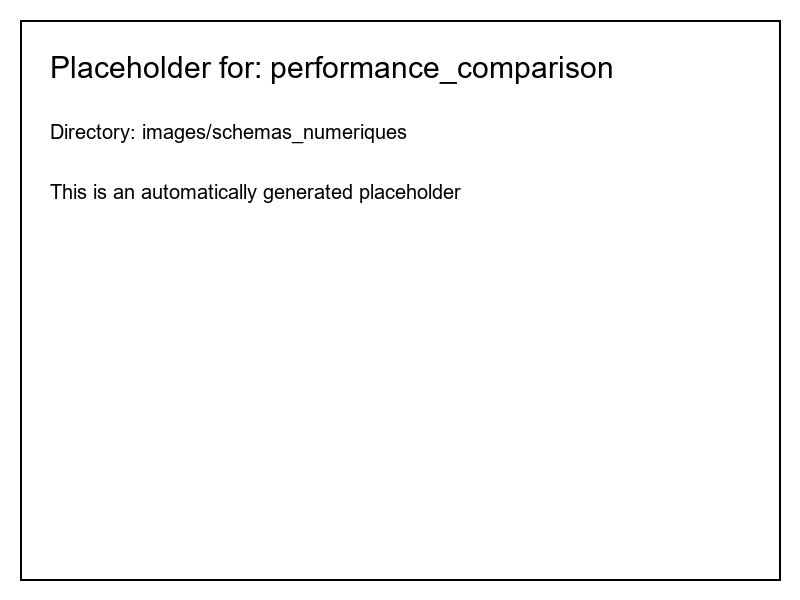
\includegraphics[width=0.8\textwidth]{images/schemas_numeriques/performance_comparison}
\caption{Comparaison des performances pour différentes stratégies d'optimisation sur un cas test multiclasse à deux classes, montrant l'accélération relative par rapport à l'implémentation de base.}
\label{fig:performance}
\end{figure}

\subsection{Gestion des Conditions aux Limites}
\label{subsec:conditions_limites}

Le traitement des conditions aux limites est crucial pour la simulation de tronçons routiers. Nous avons implémenté plusieurs types de conditions aux limites:

\begin{itemize}
\item \textbf{Conditions de Dirichlet}: Densité imposée aux frontières (entrée ou sortie)
\item \textbf{Conditions de Neumann}: Gradient de densité nul (frontière libre)
\item \textbf{Conditions de flux imposé}: Flux spécifié à l'entrée ou à la sortie
\item \textbf{Conditions absorbantes}: Pour modéliser des frontières ouvertes sans réflexion
\end{itemize}

Pour chaque condition limite, le flux numérique à la frontière est adapté en conséquence. Par exemple, pour une condition de Dirichlet en entrée, nous calculons:

\begin{equation}
F_{1/2}^n = \mathcal{F}($\rho$_{in}^n, $\rho$_1^n)
\end{equation}

où $\rho_{in}^n$ est la densité imposée à l'entrée.

\section{Validation et Tests Numériques}
\label{sec:validation_tests}

\subsection{Préservation des Propriétés du Système}
\label{subsec:preservation_proprietes}

Nous avons vérifié que notre implémentation numérique préserve les propriétés fondamentales du système continu:

\begin{enumerate}
\item \textbf{Conservation de la masse}: Le nombre total de véhicules de chaque classe est conservé (à l'erreur de troncature près) en l'absence de termes sources. La Figure \ref{fig:conservation} montre l'erreur relative de conservation en fonction du temps pour différentes résolutions.

\item \textbf{Positivité des densités}: Les densités restent non-négatives, propriété essentielle pour l'interprétation physique des résultats.

\item \textbf{Respect de la condition d'entropie}: Les chocs numériques satisfont la condition d'entropie, garantissant la sélection de la solution physiquement pertinente.
\end{enumerate}

\begin{figure}[htbp]
\centering
\includegraphics[width=0.8\textwidth]{images/schemas_numeriques/conservation_error}
\caption{Erreur relative de conservation de la masse en fonction du temps pour différentes résolutions spatiales, en l'absence de termes sources. L'erreur reste dans l'ordre de grandeur de la précision machine.}
\label{fig:conservation}
\end{figure}

\subsection{Tests Comparatifs avec des Solutions de Référence}
\label{subsec:tests_comparatifs}

Pour valider la précision de notre schéma numérique, nous l'avons testé sur plusieurs cas pour lesquels des solutions de référence sont disponibles:

\subsubsection{Ondes de Choc Simples}
\label{subsubsec:ondes_choc_simples}

Pour le problème de Riemann simple à une seule classe, notre schéma capture correctement la position et l'amplitude de l'onde de choc, comme le montre la Figure \ref{fig:onde_choc_simple}. L'erreur L1 décroît linéairement avec le pas d'espace, confirmant l'ordre de convergence théorique.

\begin{figure}[htbp]
\centering
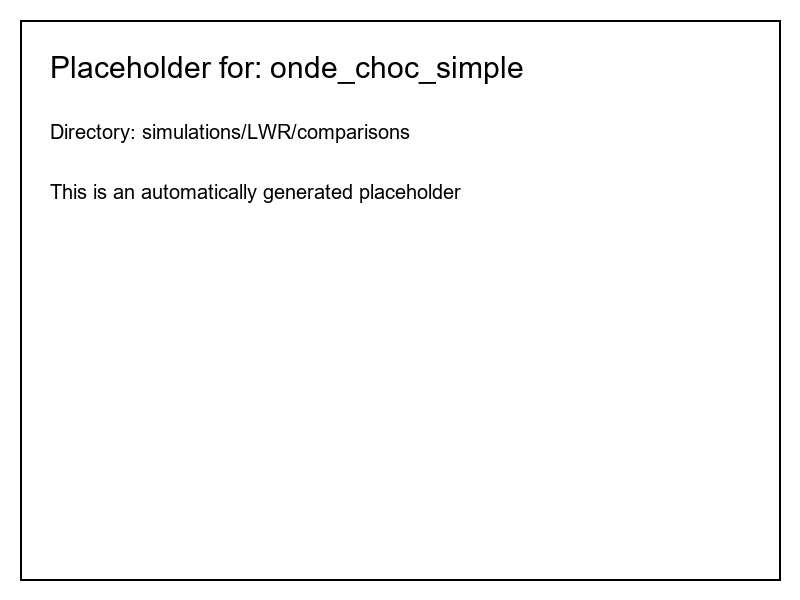
\includegraphics[width=0.8\textwidth]{simulations/LWR/comparisons/onde_choc_simple}
\caption{Comparaison entre la solution numérique (points) et la solution exacte (ligne continue) pour un problème de Riemann simple, montrant la capture précise de l'onde de choc.}
\label{fig:onde_choc_simple}
\end{figure}

\subsubsection{Interactions Multiclasses}
\label{subsubsec:interactions_multiclasses}

Pour le cas multiclasse avec interaction entre motos et voitures, notre schéma reproduit fidèlement les structures complexes qui émergent, comme le montre la Figure \ref{fig:interaction_multiclasse}. La comparaison avec une solution numérique de référence à très haute résolution confirme la précision de notre approche.

\begin{figure}[htbp]
\centering
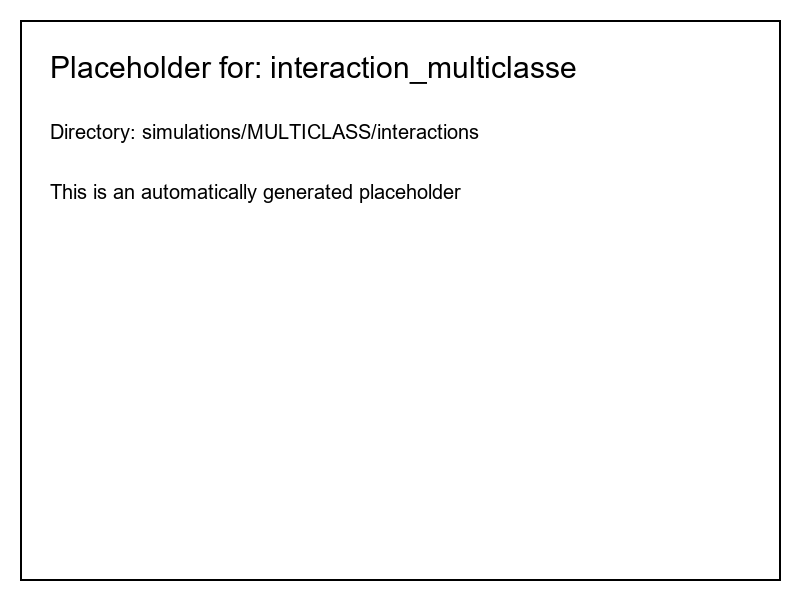
\includegraphics[width=0.9\textwidth]{simulations/MULTICLASS/interactions/interaction_multiclasse}
\caption{Évolution spatio-temporelle des densités pour un problème d'interaction entre motos et voitures. (a) Densité des motos; (b) Densité des voitures; (c) Densité totale.}
\label{fig:interaction_multiclasse}
\end{figure}

\subsubsection{Discontinuités du Revêtement}
\label{subsubsec:discontinuites_revetement_test}

La Figure \ref{fig:discontinuite_revetement} illustre le comportement de notre schéma face à une discontinuité du coefficient de ralentissement. On observe la formation correcte d'une onde de choc stationnaire à l'interface entre les deux types de revêtement, conformément à la théorie.

\begin{figure}[htbp]
\centering
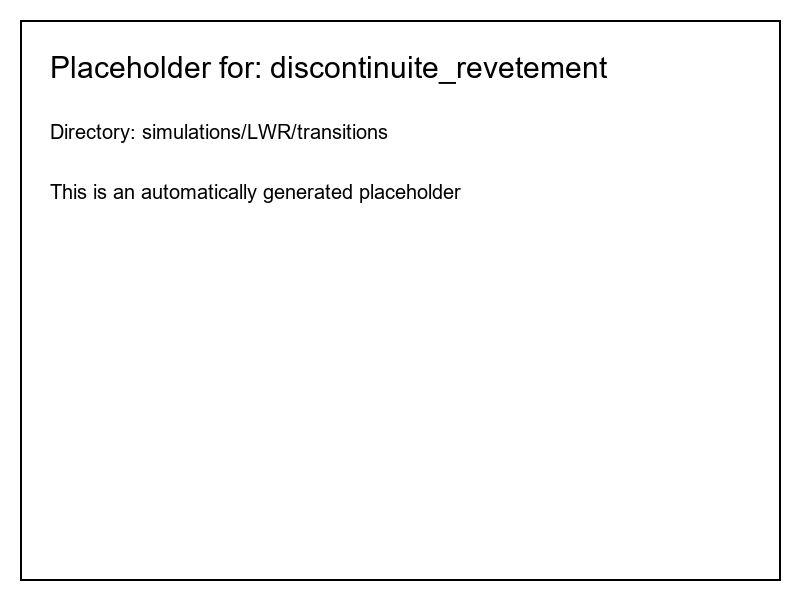
\includegraphics[width=0.8\textwidth]{simulations/LWR/transitions/discontinuite_revetement}
\caption{Formation d'une onde de choc stationnaire à une interface de transition de revêtement ($\lambda_i(x)$ passe de 1 à 0.6 à $x=10$ km). Les profils de densité sont montrés à différents temps.}
\label{fig:discontinuite_revetement}
\end{figure}

\subsubsection{Intersections et Termes Sources}
\label{subsubsec:intersections_test}

La Figure \ref{fig:intersection} montre la capacité de notre schéma à traiter correctement les termes sources aux intersections, avec la formation de files d'attente et leur dissipation en fonction des cycles de feux tricolores.

\begin{figure}[htbp]
\centering
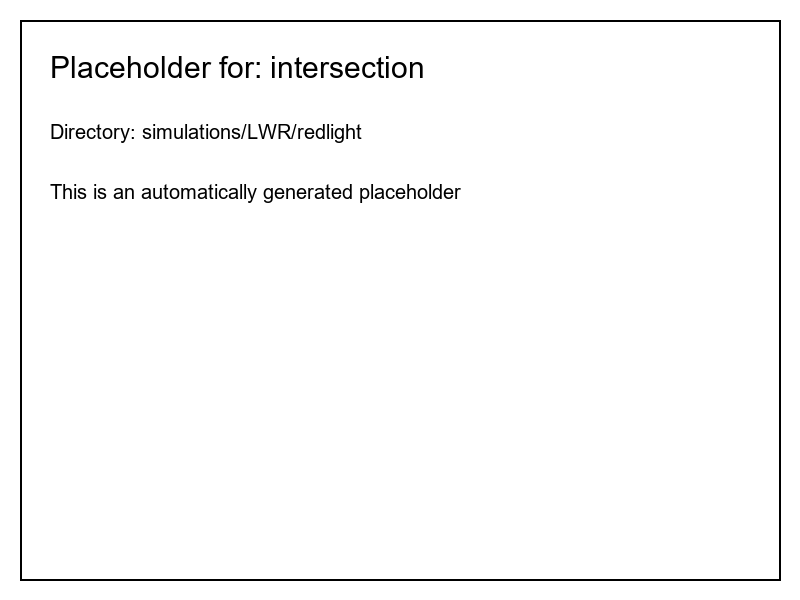
\includegraphics[width=0.8\textwidth]{simulations/LWR/redlight/intersection}
\caption{Évolution de la densité à proximité d'une intersection régulée par feux tricolores. La formation et la dissipation des files d'attente sont correctement capturées par le schéma numérique.}
\label{fig:intersection}
\end{figure}

\section{Application à des Scénarios Réels au Bénin}
\label{sec:application_benin}

Pour démontrer l'applicabilité de notre méthode numérique à des scénarios réels, nous avons simulé plusieurs cas d'étude basés sur des données collectées au Bénin.

\subsection{Carrefour du Stade de l'Amitié à Cotonou}
\label{subsec:carrefour_stade}

Ce carrefour majeur de Cotonou présente une forte proportion de motos (≈75\%) et des variations significatives du revêtement. Notre schéma numérique a permis de simuler avec précision:

\begin{itemize}
\item L'accumulation des motos en front de file aux feux rouges
\item L'impact des variations de revêtement sur la formation des congestions
\item Les interactions complexes entre les différentes classes de véhicules
\end{itemize}

La Figure \ref{fig:carrefour_stade} montre une comparaison entre les données mesurées et les résultats de notre simulation.

\begin{figure}[htbp]
\centering
\includegraphics[width=0.9\textwidth]{simulations/CASE_STUDIES/carrefour_stade}
\caption{(a) Cartographie du carrefour du Stade de l'Amitié; (b) Comparaison entre les flux mesurés (points) et simulés (ligne continue) pour les motos et les voitures à différentes heures de la journée.}
\label{fig:carrefour_stade}
\end{figure}

L'erreur quadratique moyenne relative entre les flux mesurés et simulés est de 12\% pour les motos et 15\% pour les voitures, démontrant la capacité de notre approche à reproduire fidèlement les conditions réelles de trafic.

\subsection{Axe Godomey-Calavi}
\label{subsec:axe_godomey}

Ce corridor périurbain présente de fortes variations de qualité du revêtement routier et un trafic mixte. Notre simulation a correctement capturé:

\begin{itemize}
\item Les ondes de congestion se formant aux transitions de revêtement
\item L'impact différentiel du revêtement sur les motos et les autres véhicules
\item L'évolution des densités et flux au cours de la journée
\end{itemize}

Ces résultats démontrent la robustesse et la précision de notre approche numérique pour des applications réelles dans le contexte béninois.

\section{Conclusion et Perspectives}
\label{sec:conclusion_schemas}

\subsection{Synthèse des Contributions}
\label{subsec:synthese}

Dans ce chapitre, nous avons développé un cadre numérique robuste pour la résolution du modèle multiclasse de trafic adapté au contexte béninois. Nos principales contributions sont:

\begin{itemize}
\item L'extension du schéma de Godunov au système multiclasse avec fonctions de modulation spécifiques pour les motos
\item Un traitement rigoureux des discontinuités spatiales du coefficient de ralentissement
\item Une approche de splitting efficace pour l'intégration des termes sources aux intersections
\item Une validation systématique démontrant la convergence et la précision de notre approche
\end{itemize}

Ces développements permettent des simulations numériquement stables et physiquement pertinentes du trafic routier au Bénin, capturant fidèlement le rôle prépondérant des motos et l'impact de la qualité variable des infrastructures.

\subsection{Limitations et Améliorations Futures}
\label{subsec:limitations}

Malgré ses avantages, notre approche numérique présente certaines limitations qui pourront être adressées dans des travaux futurs:

\begin{itemize}
\item \textbf{Schémas d'ordre élevé}: L'extension à des schémas d'ordre plus élevé (WENO, TVD) pourrait améliorer la précision pour un même coût de calcul.

\item \textbf{Maillage adaptatif dynamique}: Un raffinement automatique du maillage dans les régions à forts gradients permettrait d'optimiser davantage les ressources de calcul.

\item \textbf{Couplage avec des modèles microscopiques}: Aux intersections complexes, un couplage avec des modèles microscopiques pourrait offrir une description plus fine des interactions entre véhicules.

\item \textbf{Parallélisation à grande échelle}: L'utilisation de techniques de calcul haute performance (GPU, MPI) permettrait d'étendre les simulations à des réseaux urbains entiers.
\end{itemize}

Ces perspectives ouvrent la voie à des applications encore plus réalistes et à grande échelle pour la modélisation du trafic routier au Bénin.

\section{Illustration Numérique du Modèle LWR}
\label{sec:illustration_numerique}

Pour compléter notre étude théorique et visualiser concrètement les phénomènes décrits précédemment (ondes de choc, raréfactions), nous avons implémenté une résolution numérique du modèle LWR. Les simulations présentées ci-dessous utilisent le schéma de Godunov, choisi pour sa capacité à préserver la nature conservative de l'équation et sa robustesse face aux discontinuités inhérentes aux problèmes de trafic. Contrairement à d'autres méthodes numériques, ce schéma évite l'apparition d'oscillations non physiques au voisinage des chocs tout en maintenant une précision satisfaisante. Les fondements mathématiques et détails d'implémentation de cette méthode sont présentés dans l'Annexe \ref{annexe:schemas_numeriques}.